\subsection{Regressore}

\subsubsection{Dataset originale}


\noindent \textbf{Dataset completo}


\noindent Il nuovo dataset presenta i seguenti valori:
\begin{itemize}
    \item \textbf{n\_users}: [19841, 22155, 23679, 50000, 6040]
    \item \textbf{n\_items}: [42457, 24878, 33653, 38932, 54458, 4414, 10000 3706]
    \item \textbf{n\_inter}: [900212, 218457, 440620, 667850, 1465871, 1048575, 7053774, 1000209]
    \item \textbf{sparsity}: [0.99893136, 0.99955742, 0.9993401, 0.99913541, 0.99878504, 0.98996762,
    0.98589245, 0.95531637]
    \item \textbf{kg\_entities}: [50665, 32907, 42031, 47308, 26315, 0, 175646, 79347]
    \item \textbf{kg\_relations}: [5, 16, 0, 31, 49]
    \item \textbf{kg\_triples}: [46827, 29822, 38491, 43559, 96476, 0, 521125, 385923]
    \item \textbf{kg\_items}: [816701, 11446, 0, 10601, 3655]
    \item \textbf{cpu\_cores}: [12, 4]
    \item \textbf{ram\_size}: [64, 16, 27.40581512]
    \item \textbf{is\_gpu}: [1, 0]
\end{itemize}

\noindent Si può dunque notare un miglioramento per quanto riguarda la varietà dei valori rispetto al passato

\noindent I nuovi dati hanno portato alla seguente distribuzione dei dati (qui di seguito visualizzata):
\begin{figure}[H]
    \centering
    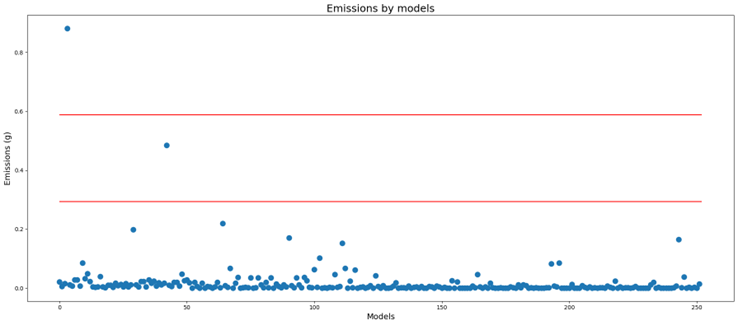
\includegraphics[width=\textwidth]{images/nuova-situazione.png}
    \caption{Distribuzione delle emissioni nel dataset completo}
\end{figure}

\noindent Come è possibile notare però, i nuovi esperimenti hanno portato a un'ulteriore sbilanciamento nel dataset, in quanto tutti gli esperimenti con DGCF e altri modelli svettano sui risultati degli altri modelli in emissioni.
Questo si riflette nei risultati ottenuti dai modelli di regressione. Per quanto riguarda i modelli,
sono stati eseguti addestramenti con diversi split tra training e test set.


\noindent\textbf{Split 50/50}

\begin{table}[H]
    \centering
    \begin{tabular}{|>{\centering\arraybackslash}m{5cm}|c|c|c|c|}
        \hline
        \textbf{Regressor} & \textbf{MAE} & \textbf{RMSE} & \textbf{MSLE} \\ [10pt]
        \hline
        SVR & 0.1053920 & 0.0207610 & 0.0131238 \\ [10pt]
        \hline
        Decision Tree & 0.0369020 & 0.0149577 & 0.0079782 \\ [10pt]
        \hline
        Random Forest & 0.0338687 & 0.0151556 & 0.0077735 \\ [10pt]
        \hline
        AdaBoost & 0.0397532 & 0.0148615 & 0.0079069 \\ [10pt]
        \hline
    \end{tabular}
    \caption{Risultati ottenuti con il nuovo dataset split 50/50}
    \label{tab:results}
\end{table}

\begin{table}[H]
    \centering
    \footnotesize
    \setlength\tabcolsep{0pt}
    \begin{tabularx}{\textwidth}{|X|X|}
        \hline
        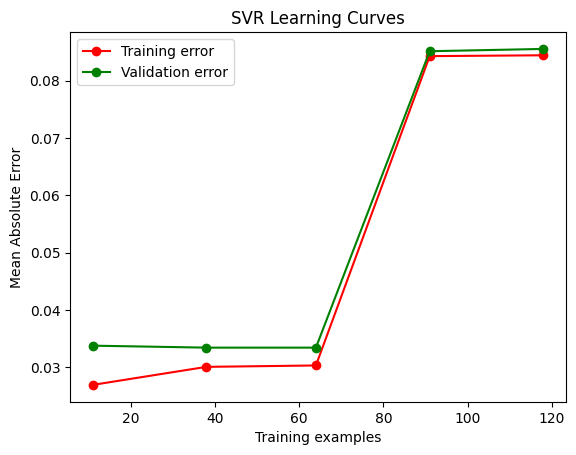
\includegraphics[width=\linewidth, trim=0 0 0 0]{images/SVR_lc50.png} &
        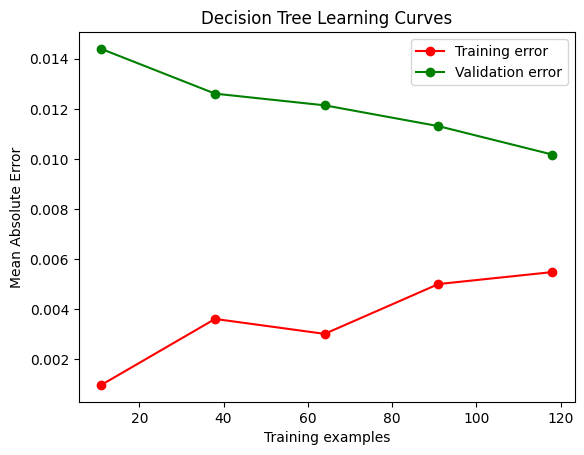
\includegraphics[width=\linewidth, trim=0 0 0 0]{images/DecisionTree_lc50.png} \\
        \hline
        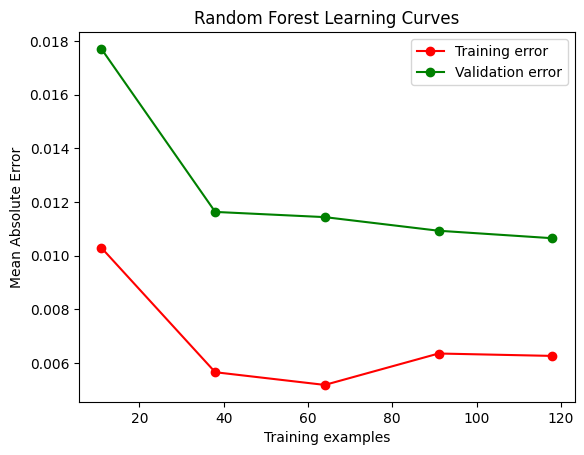
\includegraphics[width=\linewidth, trim=0 0 0 0]{images/RandomForest_lc50.png} &
        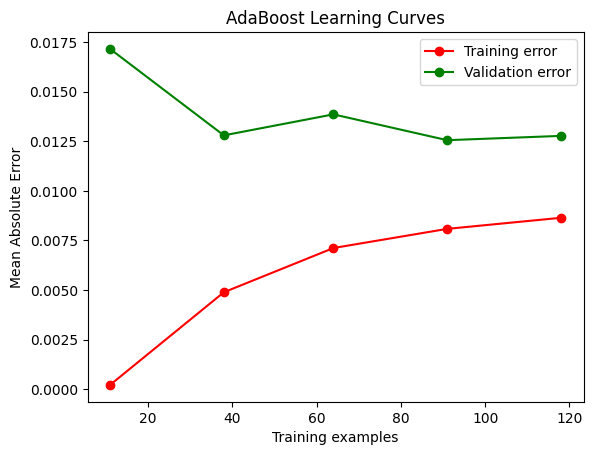
\includegraphics[width=\linewidth, trim=0 0 0 0]{images/AdaBoost_lc50.png} \\
        \hline
    \end{tabularx}
    \caption{Learning Curves con il nuovo dataset split 50/50}
    \label{tab:emissions_info}
\end{table}

\paragraph{\textbf{SVR}.}
Dal punto di vista delle metriche il regressore SVR ha ottenuto i peggiori risultati in termini di MAE, RMSE e MSLE. La learning curve mostra che il modello non è in grado di generalizzare, entrambe le curve crescono all'aumentare delle istanze.

\paragraph{\textbf{Decision Tree Regressor}.}
Dal punto di vista delle metriche, il Decision Tree Regressor ha ottenuto i risultati secondi al Random Forest Regressor. 
La learning curve mostra che la curva di training aumenta all'aumentare del numero di istanze mentre quella di validation diminuisce. Il modello dunque non ha generalizzato bene.
\paragraph{\textbf{Random Forest Regressor}.}
Dal punto di vista delle metriche il Random Forest Regressor risulta essere il miglior modello.
La learning curves di train e di validation set diminuiscono all'aumentare del numero di istanze. Quella di training tra 60 in poi aumenta ma intorno a 100 di stabilizza. Il modello sembra cominciare a generalizzare.
\paragraph{\textbf{AdaBoost Regressor}.}
Dal punto di vista delle metriche il AdaBoost Regressor ha ottenuto risultati peggiori rispetto al Decision Tree Regressor ma migliori rispetto al SVR.
La learning curve mostrano che il modello non è riuscito a generalizzare bene
in quanto la curva di validation aumenta e diminuisce all'aumentare delle istanze, mentre quella di training aumenta.

\paragraph{\textbf{Conclusioni}} Random Forest sembra essere il migliore sia dal punto di vista delle metriche che delle curve. Segue dietro il Decision Tree. AdaBoost e SVR non sono riusciti a generalizzare bene.



\noindent\textbf{Split 60/40}

\begin{table}[H]
    \centering
    \begin{tabular}{|>{\centering\arraybackslash}m{5cm}|c|c|c|c|}
        \hline
        \textbf{Regressor} & \textbf{MAE} & \textbf{RMSE} & \textbf{MSLE} \\ [10pt]
        \hline
        SVR & 0.1082652 & 0.0237656 & 0.0144029 \\ [10pt]
        \hline
        Decision Tree & 0.0439202 & 0.0183129 & 0.0096602 \\ [10pt]
        \hline
        Random Forest & 0.0405412 & 0.0188566 & 0.0096752 \\ [10pt]
        \hline
        AdaBoost & 0.0519845 & 0.0186018 & 0.0099135 \\ [10pt]
        \hline
    \end{tabular}
    \caption{Risultati ottenuti con il nuovo dataset split 60/40}
    \label{tab:results}
\end{table}

\begin{table}[H]
    \centering
    \footnotesize
    \setlength\tabcolsep{0pt}
    \begin{tabularx}{\textwidth}{|X|X|}
        \hline
        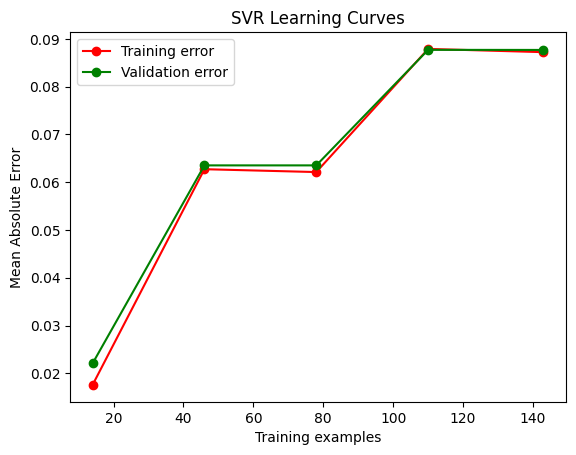
\includegraphics[width=\linewidth, trim=0 0 0 0]{images/SVR_lc60.png} &
        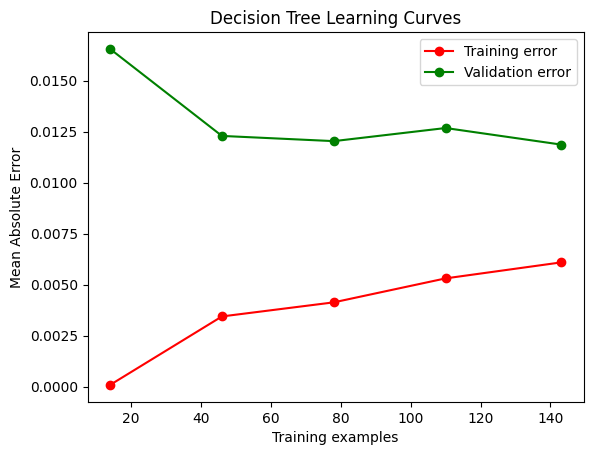
\includegraphics[width=\linewidth, trim=0 0 0 0]{images/DecisionTree_lc60.png} \\
        \hline
        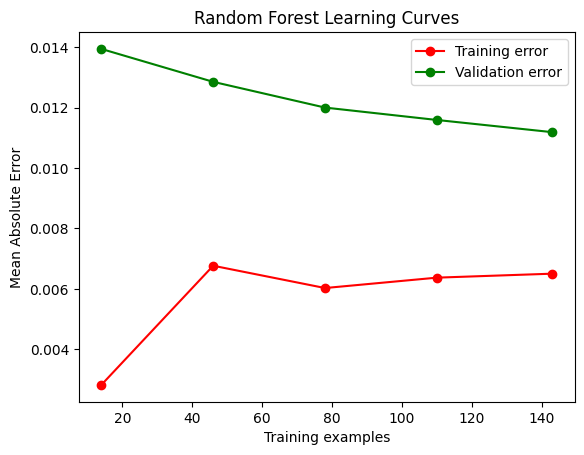
\includegraphics[width=\linewidth, trim=0 0 0 0]{images/RandomForest_lc60.png} &
        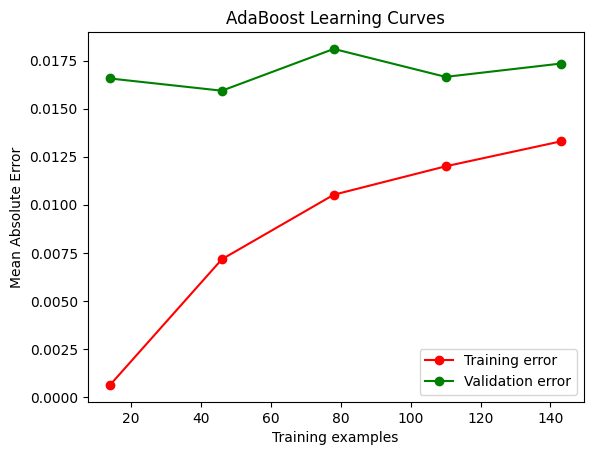
\includegraphics[width=\linewidth, trim=0 0 0 0]{images/AdaBoost_lc60.png} \\
        \hline
    \end{tabularx}
    \caption{Learning Curves con il nuovo dataset split 60/40}
    \label{tab:emissions_info}
\end{table}

\paragraph{\textbf{SVR}.}
Dal punto di vista delle metriche il regressore SVR ha ottenuto i peggiori risultati in termini di MAE, RMSE e MSLE. La learning curve mostra che il modello non è in grado di generalizzare, entrambe le curve crescono all'aumentare delle istanze.

\paragraph{\textbf{Decision Tree Regressor}.}
Dal punto di vista delle metriche, il Decision Tree Regressor ha ottenuto i risultati secondi al Random Forest Regressor. 
La learning curve mostra che la curva di training aumenta all'aumentare del numero di istanze mentre quella di validation diminuisce. Il modello dunque non ha generalizzato bene.
\paragraph{\textbf{Random Forest Regressor}.}
Dal punto di vista delle metriche il Random Forest Regressor risulta essere il miglior modello.
La learning curves di training diminuisce all'aumentare del numero di istanze. Quella di training intorno a 80 comincia ad aumentare leggermente e a stabilizzarsi.
\paragraph{\textbf{AdaBoost Regressor}.}
Dal punto di vista delle metriche il AdaBoost Regressor ha ottenuto risultati peggiori rispetto al Decision Tree Regressor ma migliori rispetto al SVR.
La learning curve mostrano che il modello non è riuscito a generalizzare bene
in quanto la curva di validation aumenta e diminuisce all'aumentare delle istanze, mentre quella di training aumenta.

\paragraph{\textbf{Conclusioni}} Random Forest sembra essere il migliore sia dal punto di vista delle metriche che delle curve. Segue dietro il Decision Tree. AdaBoost e SVR non sono riusciti a generalizzare bene. In generale i modelli peggiorano rispetto allo split 50/50.




\noindent\textbf{Split 70/30}

\begin{table}[H]
    \centering
    \begin{tabular}{|>{\centering\arraybackslash}m{5cm}|c|c|c|c|}
        \hline
        \textbf{Regressor} & \textbf{MAE} & \textbf{RMSE} & \textbf{MSLE} \\ [10pt]
        \hline
        SVR & 0.1103392 & 0.0268736 & 0.0154947 \\ [10pt]
        \hline
        Decision Tree & 0.0419923 & 0.0139534 & 0.0067713 \\ [10pt]
        \hline
        Random Forest & 0.0410102 & 0.0179366 & 0.0081916 \\ [10pt]
        \hline
        AdaBoost & 0.0486434 & 0.0160941 & 0.0074143 \\ [10pt]
        \hline
    \end{tabular}
    \caption{Risultati ottenuti con il nuovo dataset split 70/30}
    \label{tab:results} 
\end{table}

\begin{table}[H]
    \centering
    \footnotesize
    \setlength\tabcolsep{0pt}
    \begin{tabularx}{\textwidth}{|X|X|}
        \hline
        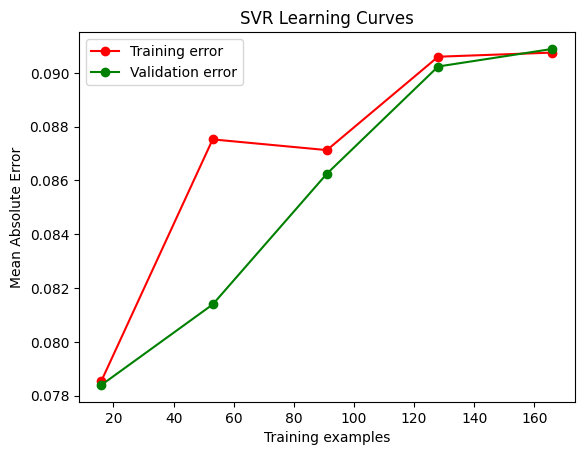
\includegraphics[width=\linewidth, trim=0 0 0 0]{images/SVR_lc70.png} &
        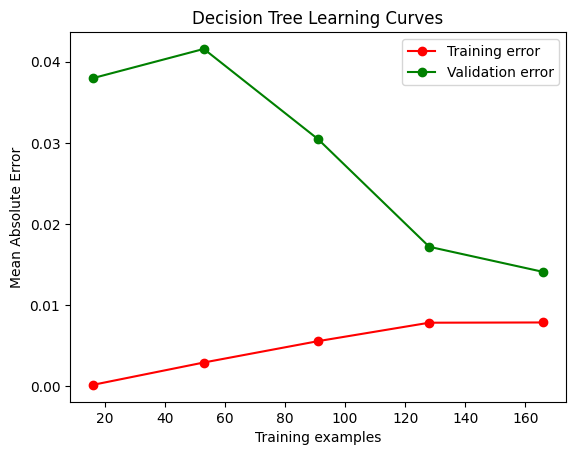
\includegraphics[width=\linewidth, trim=0 0 0 0]{images/DecisionTree_lc70.png} \\
        \hline
        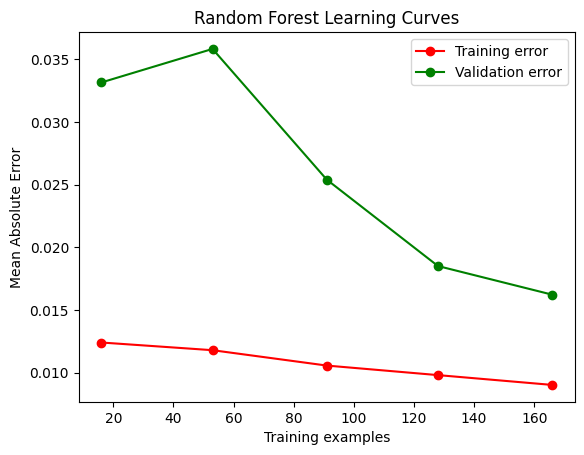
\includegraphics[width=\linewidth, trim=0 0 0 0]{images/RandomForestRegressor_lc70.png} &
        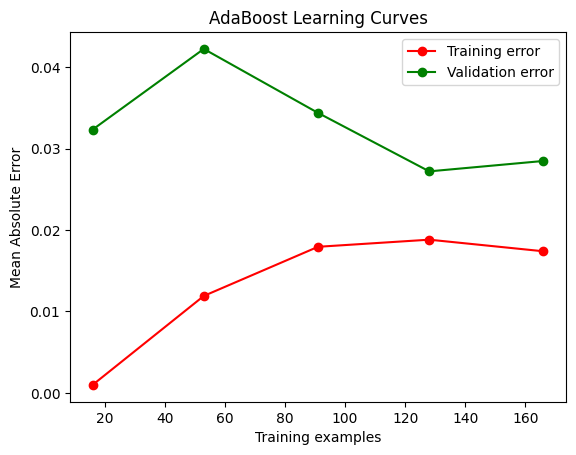
\includegraphics[width=\linewidth, trim=0 0 0 0]{images/AdaBoostRegressor_lc70.png} \\
        \hline
    \end{tabularx}
    \caption{Learning Curves con il nuovo dataset split 70/30}
    \label{tab:emissions_info}
\end{table}

\paragraph{\textbf{SVR}.}
Dal punto di vista delle metriche il regressore SVR ha ottenuto i peggiori risultati in termini di MAE, RMSE e MSLE. La learning curve mostra che il modello non è in grado di generalizare, l'errore aumenta all'aumentare delle istanze.

\paragraph{\textbf{Decision Tree Regressor}.}
Dal punto di vista delle metriche di RMSE e MSLE, il Decision Tree Regressor ha ottenuto i migliori risultati. 
La learning curve mostra una curva di training che aumenta all'aumentare del numero di istanze, mentre la curva di validation diminuisce. Le due curve si avvicinano, ma non si sovrappongono. Sembra esserci un leggero miglioramento rispetto al passato.
\paragraph{\textbf{Random Forest Regressor}.}
Dal punto di vista delle metriche il Random Forest Regressor risulta essere il secondo miglior modello, tranne per MAE dove è il migliore.
La learning curves di train e di validation set diminuiscono entrambe all'aumentare del numero di istanze, ma non si sovrappongono. Anche qui rispetto al passato si nota un leggero miglioramento.
\paragraph{\textbf{AdaBoost Regressor}.}
Dal punto di vista delle metriche il AdaBoost Regressor ha ottenuto risultati peggiori rispetto al Random Forest Regressor e al Decision Tree Regressor ma migliori rispetto al SVR.
La learning curve mostrano che il modello non è riuscito a generalizzare bene ma si è comportato meglio rispetto al passato.


\paragraph{\textbf{Conclusioni}} Vi è un generale miglioramento rispetto allo split 60/40. Random Forest e Decision Tree sono i migliori modelli. AdaBoost e SVR non sono riusciti a generalizzare bene.



\noindent\textbf{Split 80/20}

\begin{table}[H]
    \centering
    \begin{tabular}{|>{\centering\arraybackslash}m{5cm}|c|c|c|c|}
        \hline
        \textbf{Regressor} & \textbf{MAE} & \textbf{RMSE} & \textbf{MSLE} \\ [10pt]
        \hline
        SVR & 0.1211949 & 0.0364312 & 0.0196837 \\ [10pt]
        \hline
        Decision Tree & 0.0511053 & 0.0211890 & 0.0095072 \\ [10pt]
        \hline
        Random Forest & 0.0538403 & 0.0262660 & 0.0118334 \\ [10pt]
        \hline
        AdaBoost & 0.0617220 & 0.0230938 & 0.0104140 \\ [10pt]
        \hline
    \end{tabular}
    \caption{Risultati ottenuti con il nuovo dataset split 80/20}
    \label{tab:results} 
\end{table}

\begin{table}[H]
    \centering
    \footnotesize
    \setlength\tabcolsep{0pt}
    \begin{tabularx}{\textwidth}{|X|X|}
        \hline
        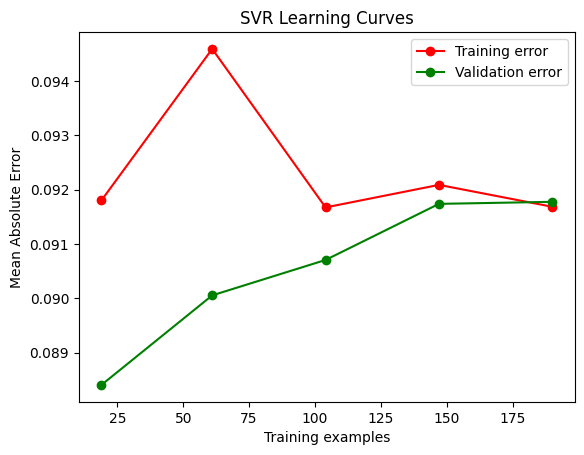
\includegraphics[width=\linewidth, trim=0 0 0 0]{images/SVR_lc80.png} &
        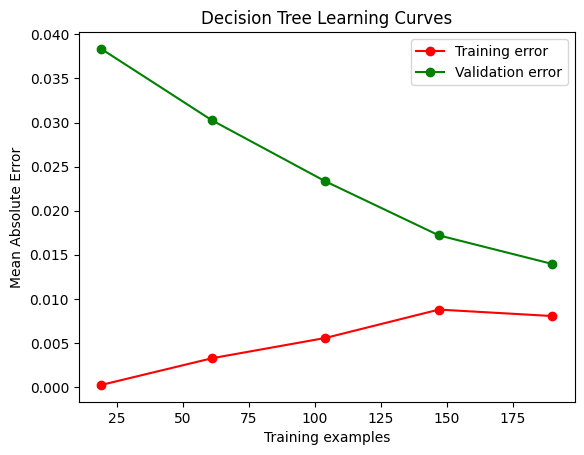
\includegraphics[width=\linewidth, trim=0 0 0 0]{images/DecisionTree_lc80.png} \\
        \hline
        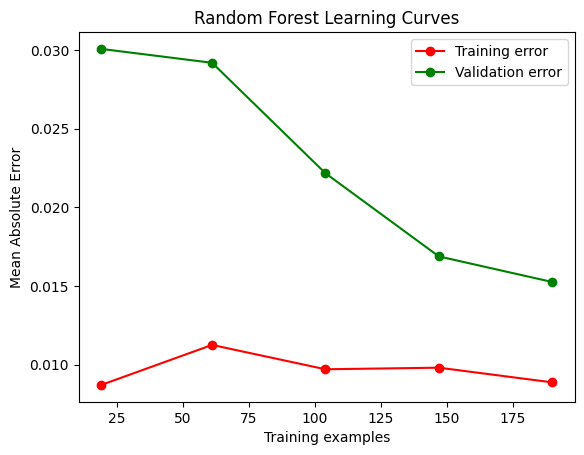
\includegraphics[width=\linewidth, trim=0 0 0 0]{images/RandomForest_lc80.png} &
        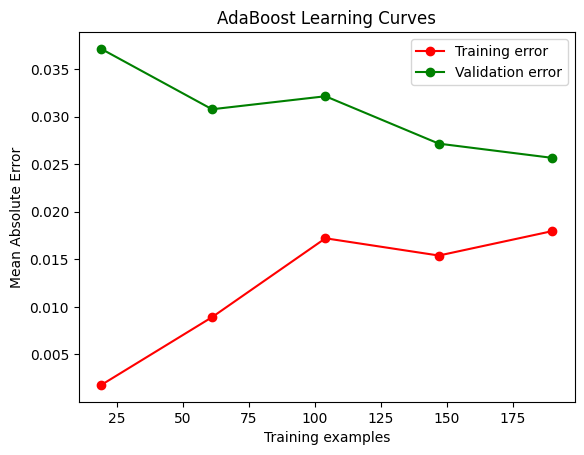
\includegraphics[width=\linewidth, trim=0 0 0 0]{images/AdaBoost_lc80.png} \\
        \hline
    \end{tabularx}
    \caption{Learning Curves con il nuovo dataset split 80/20}
    \label{tab:emissions_info}
\end{table}

\paragraph{\textbf{SVR}.}
Dal punto di vista delle metriche il regressore SVR ha ottenuto i peggiori risultati in termini di MAE, RMSE e MSLE. La learning curve di validation aumenta all'aumentare delle istanze, mentre quella di training è più instabile. Il modello non è riuscito a generalizzare bene.

\paragraph{\textbf{Decision Tree Regressor}.}
Dal punto di vista delle metriche il Decision Tree Regressor ha ottenuto i migliori risultati. 
La learning curve mostra una curva di training che aumenta all'aumentare del numero di istanze cominciando una lenta discesa verso le 150 istanze, mentre la curva di validation diminuisce. Le due curve si avvicinano, Sembra che il modello cominci a generalizzare.
\paragraph{\textbf{Random Forest Regressor}.}
Random Forest Regressor è secondo migliore in MAE, terzo in RMSE e MSLE.
La learning curves di train e di validation set diminuiscono entrambe all'aumentare del numero di istanze, ma non si sovrappongono. Comportamento analogo al passato.
\paragraph{\textbf{AdaBoost Regressor}.}
AdaBoost è il secondo migliore in RMSE e MSLE, terzo in MAE.
La learning curve mostrano che il modello non è riuscito a generalizzare bene.


\paragraph{\textbf{Conclusioni}} Decision Tree è il miglior modello. Tuttavia rispetto allo split precedente vi è un generale peggioramento delle performance.

\noindent\textbf{Split 90/10}

\begin{table}[H]
    \centering
    \begin{tabular}{|>{\centering\arraybackslash}m{5cm}|c|c|c|c|}
        \hline
        \textbf{Regressor} & \textbf{MAE} & \textbf{RMSE} & \textbf{MSLE} \\ [10pt]
        \hline
        SVR & 0.1193075 & 0.0308946 & 0.0181817 \\ [10pt]
        \hline
        Decision Tree & 0.1011067 & 0.0860050 & 0.0377845 \\ [10pt]
        \hline
        Random Forest & 0.0857748 & 0.0539394 & 0.0275298 \\ [10pt]
        \hline
        AdaBoost & 0.1282122 & 0.0921047 & 0.0410386 \\ [10pt]
        \hline
    \end{tabular}
    \caption{Risultati ottenuti con il nuovo dataset split 90/10}
    \label{tab:results} 
\end{table}

\begin{table}[H]
    \centering
    \footnotesize
    \setlength\tabcolsep{0pt}
    \begin{tabularx}{\textwidth}{|X|X|}
        \hline
        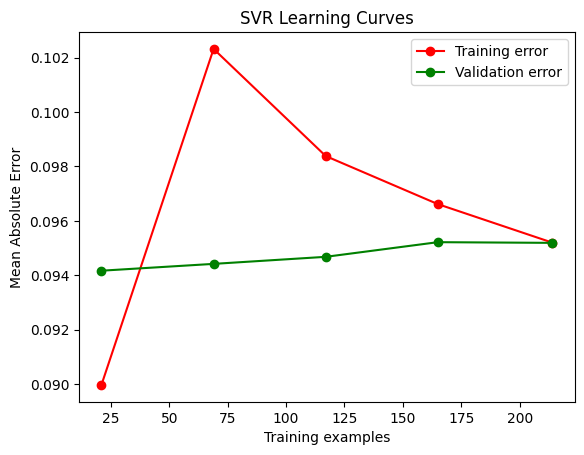
\includegraphics[width=\linewidth, trim=0 0 0 0]{images/SVR_lc90.png} &
        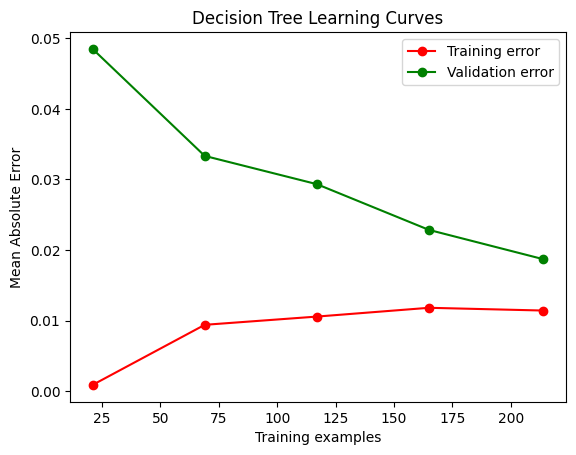
\includegraphics[width=\linewidth, trim=0 0 0 0]{images/DecisionTree_lc90.png} \\
        \hline
        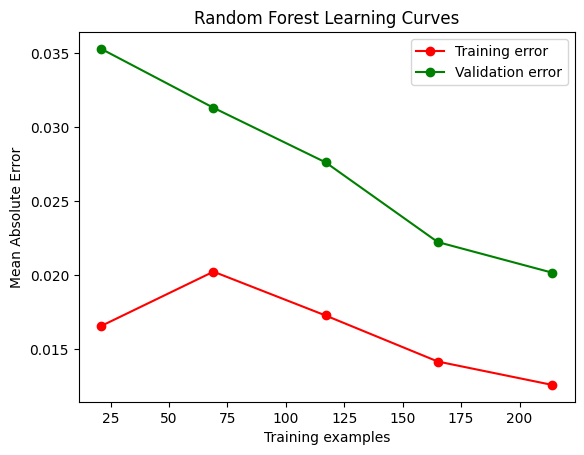
\includegraphics[width=\linewidth, trim=0 0 0 0]{images/RandomForest_lc90.png} &
        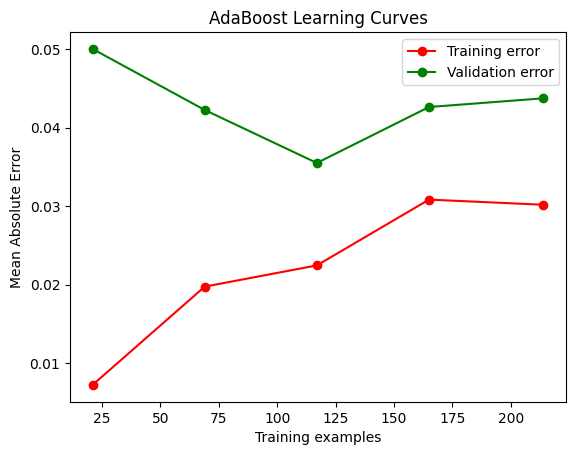
\includegraphics[width=\linewidth, trim=0 0 0 0]{images/AdaBoost_lc90.png} \\
        \hline
    \end{tabularx}
    \caption{Learning Curves con il nuovo dataset split 90/10}
    \label{tab:emissions_info}
\end{table}

\paragraph{\textbf{SVR}.}
Dal punto di vista delle metriche il regressore SVR ha un pessimo risultato in MAE ma ha i migliori risultati in RMSE e MSLE. La learning curve di validation aumenta all'aumentare delle istanze, mentre quella di training è più instabile. Il modello non è riuscito a generalizzare bene.

\paragraph{\textbf{Decision Tree Regressor}.}
Dal punto di vista delle metriche, Decision è il secondo miglior modello.
La learning curve mostra una curva di training che aumenta all'aumentare del numero di istanze, mentre la curva di validation diminuisce. Le due curve si avvicinano, ma non si sovrappongono. Comportamento analogo al passato.
\paragraph{\textbf{Random Forest Regressor}.}
Dal punto di vista delle metriche il Random Forest Regressor risulta essere il miglior modello.
La learning curves di train e di validation set diminuiscono entrambe all'aumentare del numero di istanze, ma non si sovrappongono. Comportamento analogo al passato.
\paragraph{\textbf{AdaBoost Regressor}.}
Dal punto di vista delle metriche il AdaBoost Regressor ha ottenuto i risultati peggiori.
La learning curve mostrano che il modello non è riuscito a generalizzare bene in quanto entrambe le curve crescono all'aumentare delle istanze.


\paragraph{\textbf{Conclusioni}} Il miglior modello si conferma Random Forest. Il secondo migliore sembra essere SVR. In generale vi è un drastico peggioramento delle performance rispetto allo split precedente.



\paragraph{\textbf{Conclusioni generali}} 
In generale Random Forest sembra essere il miglior modello. Decision Tree è il secondo migliore. AdaBoost e SVR non sono riusciti a generalizzare bene. In particolare lo split dove le performance sono migliori osservando sia learning curve che metriche è il 70/30 a cui segue il 60/40.



\subsubsection{Dataset Azure}


\noindent Parallelamente si è deciso di procedere eliminando tutti i risultati non prodotti sulla macchina Azure in modo da avere un regressore specifico per tali esperimenti.

\begin{figure}[H]
    \centering
    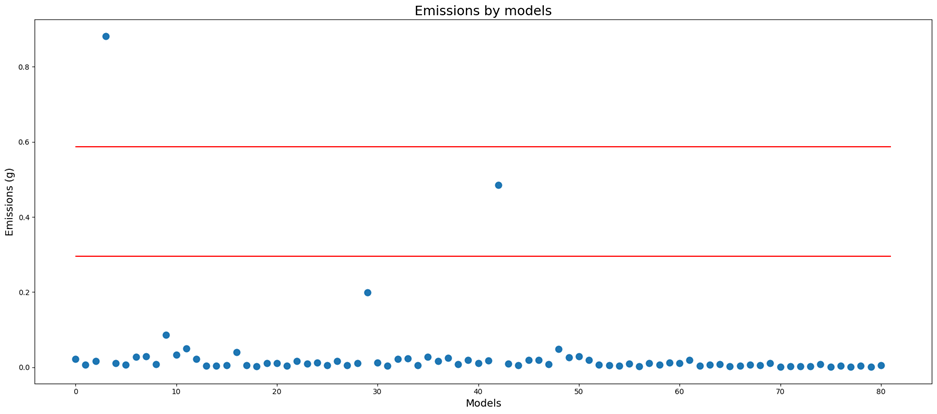
\includegraphics[width=\textwidth]{images/nuova-situazione2.png}
    \caption{Distribuzione delle emissioni nel dataset Azure}
\end{figure}


\noindent Anche qui si è deciso di eseguire addestramenti con diversi split tra training e test set.

\noindent\textbf{Split 50/50}

\begin{table}[H]
    \centering
    \begin{tabular}{|>{\centering\arraybackslash}m{5cm}|c|c|c|c|}
        \hline
        \textbf{Regressor} & \textbf{MAE} & \textbf{RMSE} & \textbf{MSLE} \\ [10pt]
        \hline
        SVR & 0.1043015 & 0.0213416 & 0.0133855 \\ [10pt]
        \hline
        Decision Tree & 0.0583675 & 0.0329582 & 0.0154626 \\ [10pt]
        \hline
        Random Forest & 0.0459593 & 0.0179844 & 0.0092711 \\ [10pt]
        \hline
        AdaBoost & 0.0615526 & 0.0331120 & 0.0155884 \\ [10pt]
        \hline
    \end{tabular}
    \caption{Risultati ottenuti con il nuovo dataset Azure con split 50/50}
    \label{tab:results}
\end{table}

\begin{table}[H]
    \centering
    \footnotesize
    \setlength\tabcolsep{0pt}
    \begin{tabularx}{\textwidth}{|X|X|}
        \hline
        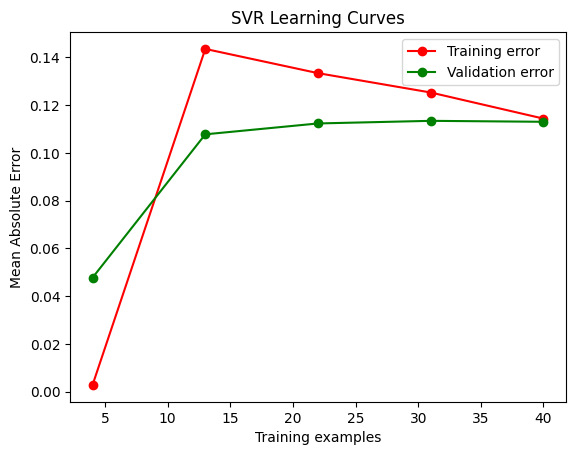
\includegraphics[width=\linewidth, trim=0 0 0 0]{images/SVR_lc50_Azure.png} &
        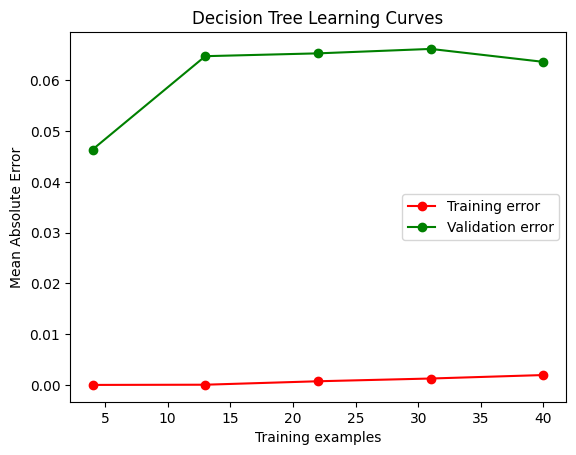
\includegraphics[width=\linewidth, trim=0 0 0 0]{images/DecisionTree_lc50_Azure.png} \\
        \hline
        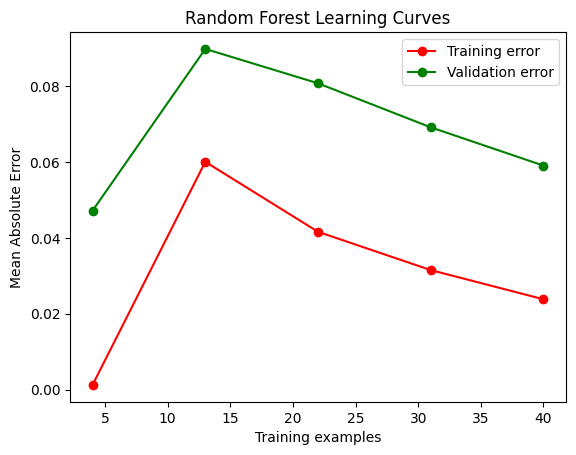
\includegraphics[width=\linewidth, trim=0 0 0 0]{images/RandomForest_lc50_Azure.png} &
        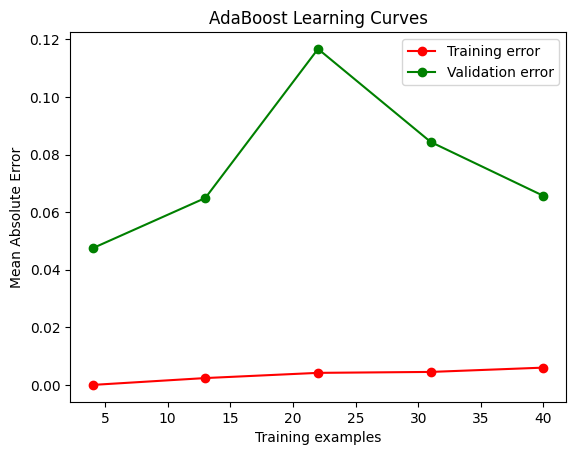
\includegraphics[width=\linewidth, trim=0 0 0 0]{images/AdaBoost_lc50_Azure.png} \\
        \hline
    \end{tabularx}
    \caption{Learning Curves con il nuovo dataset Azure con split 50/50}
    \label{tab:emissions_info}
\end{table}

\paragraph{\textbf{SVR}.}
Dal punto di vista delle metriche il regressore SVR ha ottenuto i peggiori risultati in termini di MAE e i secondi migliori in RMSE e MSLE. La training curve inizialmente cresce velocemente per poi diminuire, mentre quella di validation cresce all'aumentare delle istanze. Le due arrivano a sovrapporsi ma non si incrociano. Il modello non sembra aver generallizato bene.

\paragraph{\textbf{Decision Tree Regressor}.}
Dal punto di vista delle metriche il DecisionTree non si comporta bene. L'errore sul training è molto basso mentre sul validation è molto alto. Il modello non ha generalizzato bene.
\paragraph{\textbf{Random Forest Regressor}.}
Dal punto di vista delle metriche il Random Forest Regressor risulta essere il miglior modello.
La learning curves di train e di validation hanno lo stesso andamento e dalle 10 istanze circa in poi diminuiscono all'aumentare del numero delle istanze. Il modello generalizza meglio degli altri.
\paragraph{\textbf{AdaBoost Regressor}.}
AdaBoost dal punto di vista delle metriche è l secondo peggior modello. La learning curve mostra che il modello non è riuscito a generalizzare bene in quanto molto irregolari.

\paragraph{\textbf{Conclusioni}} RandomForest sembra essere il miglior modello. Dal punto di vista delle metriche segue Decision Tree anche se le curve non mostrano una buona generalizzazione.
\noindent\textbf{Split 60/40}

\begin{table}[H]
    \centering
    \begin{tabular}{|>{\centering\arraybackslash}m{5cm}|c|c|c|c|}
        \hline
        \textbf{Regressor} & \textbf{MAE} & \textbf{RMSE} & \textbf{MSLE} \\ [10pt]
        \hline
        SVR & 0.1097324 & 0.0248018 & 0.0150739 \\ [10pt]
        \hline
        Decision Tree & 0.0556196 & 0.0342894 & 0.0152874 \\ [10pt]
        \hline
        Random Forest & 0.0498345 & 0.0213098 & 0.0107539 \\ [10pt]
        \hline
        AdaBoost & 0.0754194 & 0.0411506 & 0.0193612 \\ [10pt]
        \hline
    \end{tabular}
    \caption{Risultati ottenuti con il nuovo dataset Azure con split 60/40}
    \label{tab:results}
\end{table}

\begin{table}[H]
    \centering
    \footnotesize
    \setlength\tabcolsep{0pt}
    \begin{tabularx}{\textwidth}{|X|X|}
        \hline
        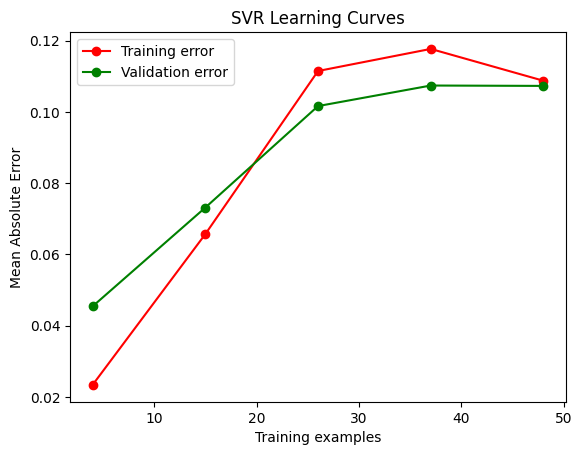
\includegraphics[width=\linewidth, trim=0 0 0 0]{images/SVR_lc60_Azure.png} &
        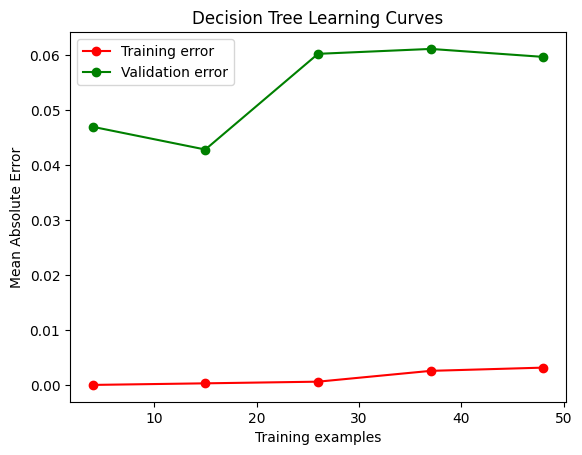
\includegraphics[width=\linewidth, trim=0 0 0 0]{images/DecisionTree_lc60_Azure.png} \\
        \hline
        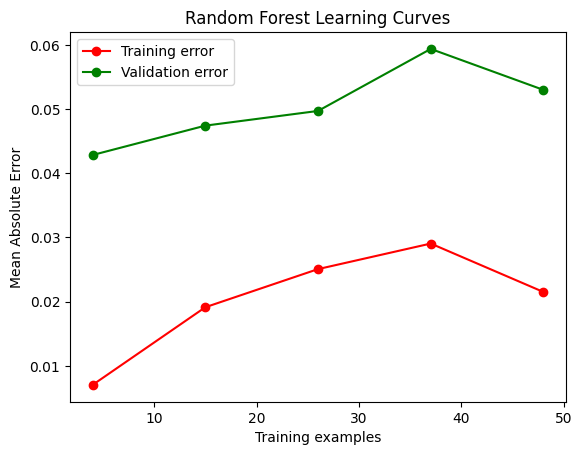
\includegraphics[width=\linewidth, trim=0 0 0 0]{images/RandomForest_lc60_Azure.png} &
        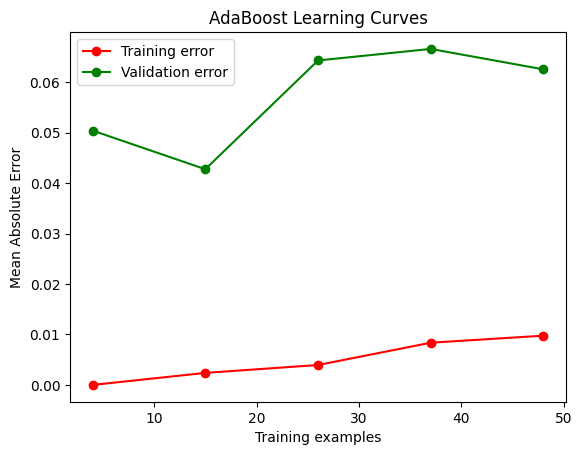
\includegraphics[width=\linewidth, trim=0 0 0 0]{images/AdaBoost_lc60_Azure.png} \\
        \hline
    \end{tabularx}
    \caption{Learning Curves con il nuovo dataset Azure con split 60/40}
    \label{tab:emissions_info}
\end{table}

\paragraph{\textbf{SVR}.}
Dal punto di vista delle metriche il regressore SVR ha ottenuto i peggiori risultati in termini di MAE e i secondi migliori in RMSE e MSLE. La training curve inizialmente cresce velocemente per poi diminuire, mentre quella di validation cresce all'aumentare delle istanze. Le due arrivano a sovrapporsi ma non si incrociano. Il modello non sembra aver generallizato bene.

\paragraph{\textbf{Decision Tree Regressor}.}
Dal punto di vista delle metriche il DecisionTree non si comporta bene. L'errore sul training è molto basso mentre sul validation è molto alto. Il modello non ha generalizzato bene.
\paragraph{\textbf{Random Forest Regressor}.}
Dal punto di vista delle metriche il Random Forest Regressor risulta essere il miglior modello.
La learning curves di train e di validation hanno lo stesso andamento e dalle 35 istanze circa in poi diminuiscono all'aumentare del numero delle istanze. Il modello generalizza meglio degli altri.
\paragraph{\textbf{AdaBoost Regressor}.}
AdaBoost dal punto di vista delle metriche è l secondo peggior modello. La learning curve mostra che il modello non è riuscito a generalizzare bene in quanto molto irregolari.

\paragraph{\textbf{Conclusioni}} RandomForest sembra essere il miglior modello. Dal punto di vista delle metriche segue Decision Tree anche se le curve non mostrano una buona generalizzazione. In generale si nota un peggioramento rispetto allo split precedente.



\noindent\textbf{Split 70/30}

\begin{table}[H]
    \centering
    \begin{tabular}{|>{\centering\arraybackslash}m{5cm}|c|c|c|c|}
        \hline
        \textbf{Regressor} & \textbf{MAE} & \textbf{RMSE} & \textbf{MSLE} \\ [10pt]
        \hline
        SVR & 0.1165169 & 0.0301642 & 0.0175917 \\ [10pt]
        \hline
        Decision Tree & 0.0691471 & 0.0450743 & 0.0199880 \\ [10pt]
        \hline
        Random Forest & 0.0641987 & 0.0306766 & 0.0153200 \\ [10pt]
        \hline
        AdaBoost & 0.0910959 & 0.0542499 & 0.0254505 \\ [10pt]
        \hline
    \end{tabular}
    \caption{Risultati ottenuti con il nuovo dataset Azure}
    \label{tab:results}
\end{table}

\begin{table}[H]
    \centering
    \footnotesize
    \setlength\tabcolsep{0pt}
    \begin{tabularx}{\textwidth}{|X|X|}
        \hline
        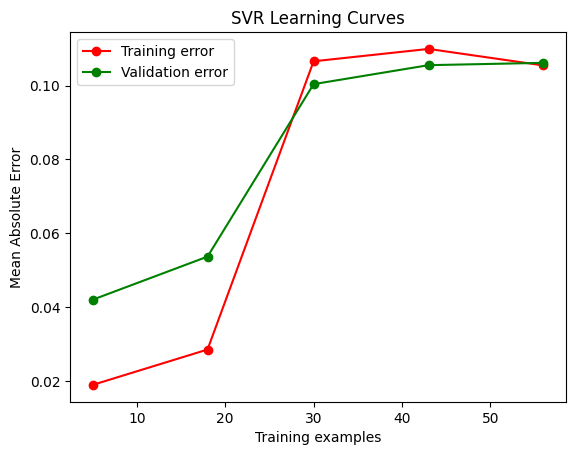
\includegraphics[width=\linewidth, trim=0 0 0 0]{images/SVR_lc70_Azure.png} &
        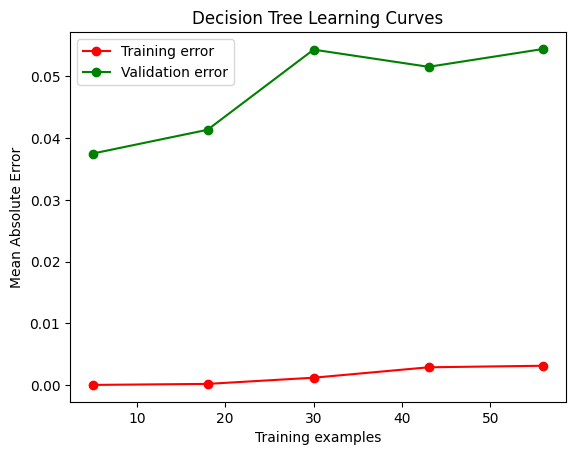
\includegraphics[width=\linewidth, trim=0 0 0 0]{images/DecisionTree_lc70_Azure.png} \\
        \hline
        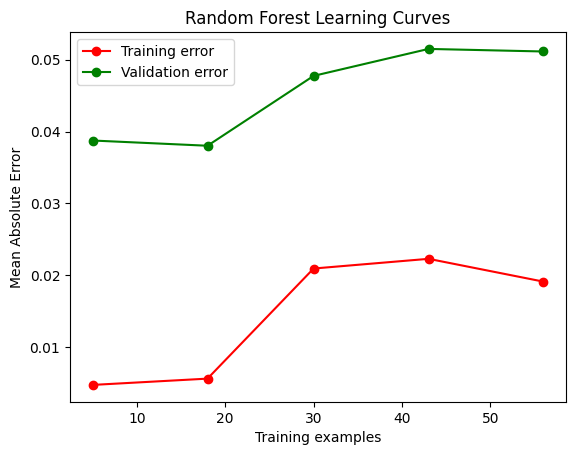
\includegraphics[width=\linewidth, trim=0 0 0 0]{images/RandomForestRegressor_lc70_Azure.png} &
        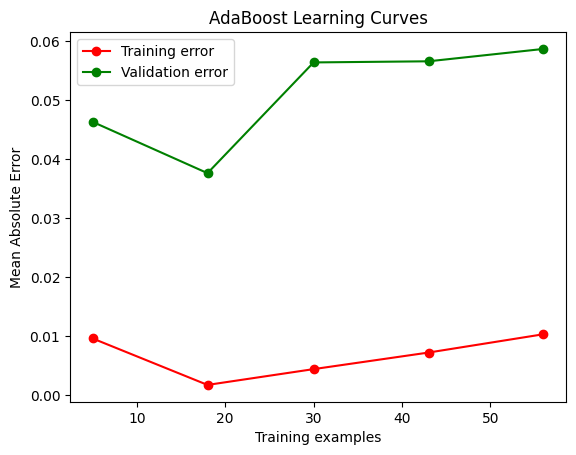
\includegraphics[width=\linewidth, trim=0 0 0 0]{images/AdaBoostRegressor_lc70_Azure.png} \\
        \hline
    \end{tabularx}
    \caption{Learning Curves con il nuovo dataset Azure}
    \label{tab:emissions_info}
\end{table}

\paragraph{\textbf{SVR}.}
Dal punto di vista delle metriche il regressore SVR ha ottenuto i peggiori risultati in termini di MAE, RMSE e MSLE. La learning curve mostra che il modello non è in grado di generalizzare, infatti l'errore di training supera anche quello di validation.

\paragraph{\textbf{Decision Tree Regressor}.}
Dal punto di vista delle metriche, il Decision Tree Regressor ha ottenuto i risultati secondi al Random Forest Regressor. 
La learning curve mostra che entrambe le curve di training e di validation aumentano all'aumentare del numero di istanze. Il modello dunque non ha generalizzato bene.
\paragraph{\textbf{Random Forest Regressor}.}
Dal punto di vista delle metriche il Random Forest Regressor risulta essere il miglior modello.
La learning curves di train e di validation set crescono all'aumentare del numero delle istanze, quella di training infine comincia una lenta discesa. Il modello comunque non ha appreso bene.
\paragraph{\textbf{AdaBoost Regressor}.}
Dal punto di vista delle metriche il AdaBoost Regressor ha ottenuto risultati peggiori rispetto al Decision Tree Regressor ma migliori rispetto al SVR.
La learning curve mostrano che il modello non è riuscito a generalizzare bene

\paragraph{\textbf{Conclusioni}} RandomForest sembra essere il miglior modello. Decision Tree è il secondo migliore. AdaBoost e SVR non sono riusciti a generalizzare bene. In generale si nota un peggioramento rispetto allo split precedente.


\noindent\textbf{Split 80/20}

\begin{table}[H]
    \centering
    \begin{tabular}{|>{\centering\arraybackslash}m{5cm}|c|c|c|c|}
        \hline
        \textbf{Regressor} & \textbf{MAE} & \textbf{RMSE} & \textbf{MSLE} \\ [10pt]
        \hline
        SVR & 0.1308274 & 0.0407490 & 0.0226068 \\ [10pt]
        \hline
        Decision Tree & 0.0470062 & 0.0118862 & 0.0057503 \\ [10pt]
        \hline
        Random Forest & 0.0557055 & 0.0218310 & 0.0098565 \\ [10pt]
        \hline
        AdaBoost & 0.0822472 & 0.0254612 & 0.0138452 \\ [10pt]
        \hline
    \end{tabular}
    \caption{Risultati ottenuti con il nuovo dataset Azure con split 80/20}
    \label{tab:results}
\end{table}

\begin{table}[H]
    \centering
    \footnotesize
    \setlength\tabcolsep{0pt}
    \begin{tabularx}{\textwidth}{|X|X|}
        \hline
        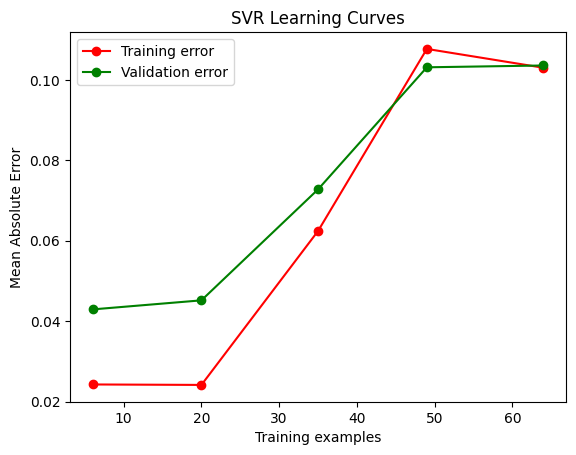
\includegraphics[width=\linewidth, trim=0 0 0 0]{images/SVR_lc80_Azure.png} &
        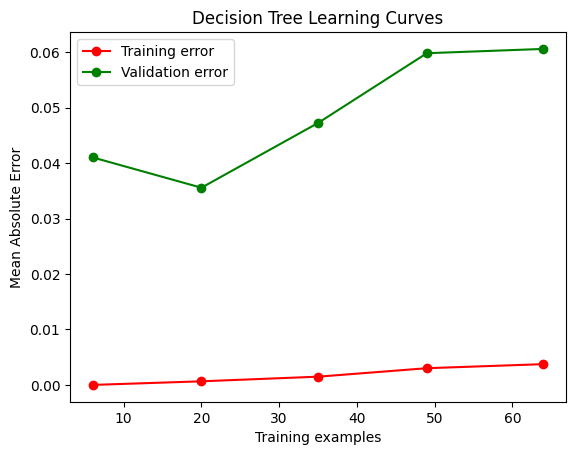
\includegraphics[width=\linewidth, trim=0 0 0 0]{images/DecisionTree_lc80_Azure.png} \\
        \hline
        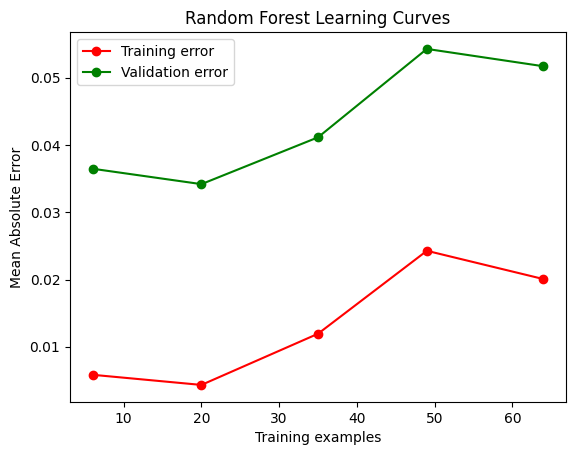
\includegraphics[width=\linewidth, trim=0 0 0 0]{images/RandomForest_lc80_Azure.png} &
        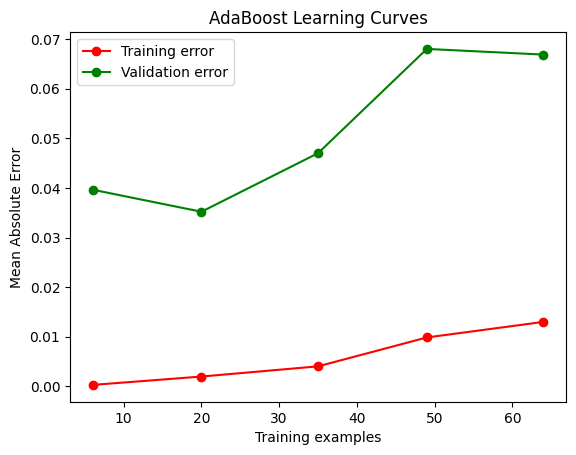
\includegraphics[width=\linewidth, trim=0 0 0 0]{images/AdaBoost_lc80_Azure.png} \\
        \hline
    \end{tabularx}
    \caption{Learning Curves con il nuovo dataset Azure con split 80/20}
    \label{tab:emissions_info}
\end{table}

\paragraph{\textbf{SVR}.}
Dal punto di vista delle metriche il regressore SVR ha ottenuto i peggiori risultati in termini di MAE, RMSE e MSLE. La learning curve mostra che il modello non è in grado di generalizzare, infatti l'errore di training supera anche quello di validation.

\paragraph{\textbf{Decision Tree Regressor}.}
Dal punto di vista delle metriche, il Decision Tree Regressor ha ottenuto i migliori risultati.
La learning curve mostra che entrambe le curve di training e di validation aumentano all'aumentare del numero di istanze. Il modello dunque non ha generalizzato bene.
\paragraph{\textbf{Random Forest Regressor}.}
Dal punto di vista delle metriche il Random Forest Regressor risulta essere il secondo miglior modello.
La learning curves di train e di validation set seguono lo stesso andamento, crescendo fino a 50 istanze e cominciando poi a diminuire. Il Comportamento è analogo al passato.
\paragraph{\textbf{AdaBoost Regressor}.}
Dal punto di vista delle metriche il AdaBoost Regressor ha ottenuto risultati peggiori rispetto al Random Forest Regressor ma migliori rispetto al SVR.
La learning curve mostrano che il modello non è riuscito a generalizzare ben in quanto entrambe le curve crescono all'aumentare delle istanze.

\paragraph{\textbf{Conclusioni}} DecisionTree è il miglior modello dal punto di vista delle metriche, il secondo migliore è Random Forest. Dal punto di vista delle curve quelle della Random Forest sono le migliori. Si nota un netto miglioramento rispetto allo split precedente.

\noindent\textbf{Split 90/10}

\begin{table}[H]
    \centering
    \begin{tabular}{|>{\centering\arraybackslash}m{5cm}|c|c|c|c|}
        \hline
        \textbf{Regressor} & \textbf{MAE} & \textbf{RMSE} & \textbf{MSLE} \\ [10pt]
        \hline
        SVR & 0.0896299 & 0.0081883 & 0.0073278 \\ [10pt]
        \hline
        Decision Tree & 0.0220335 & 0.0025806 & 0.0020781 \\ [10pt]
        \hline
        Random Forest & 0.0231489 & 0.0023014 & 0.0018764 \\ [10pt]
        \hline
        AdaBoost & 0.0384317 & 0.0063016 & 0.0047659 \\ [10pt]
        \hline
    \end{tabular}
    \caption{Risultati ottenuti con il nuovo dataset Azure con split 90/10}
    \label{tab:results}
\end{table}

\begin{table}[H]
    \centering
    \footnotesize
    \setlength\tabcolsep{0pt}
    \begin{tabularx}{\textwidth}{|X|X|}
        \hline
        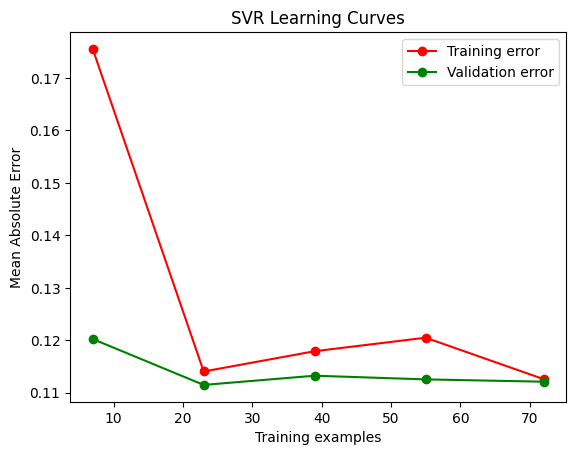
\includegraphics[width=\linewidth, trim=0 0 0 0]{images/SVR_lc90_Azure.png} &
        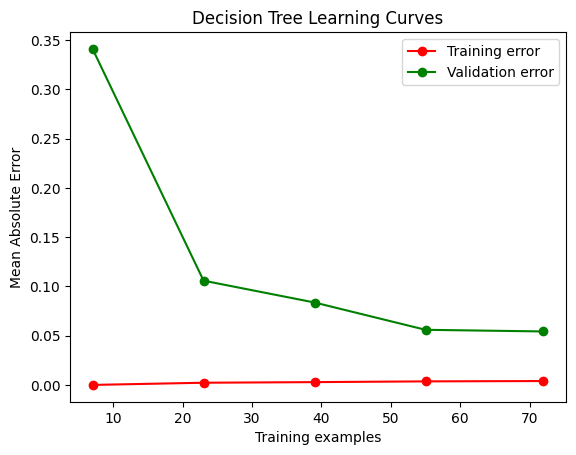
\includegraphics[width=\linewidth, trim=0 0 0 0]{images/DecisionTree_lc90_Azure.png} \\
        \hline
        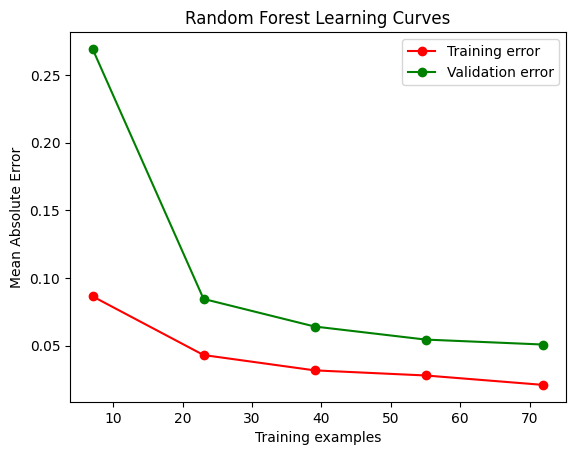
\includegraphics[width=\linewidth, trim=0 0 0 0]{images/RandomForest_lc90_Azure.png} &
        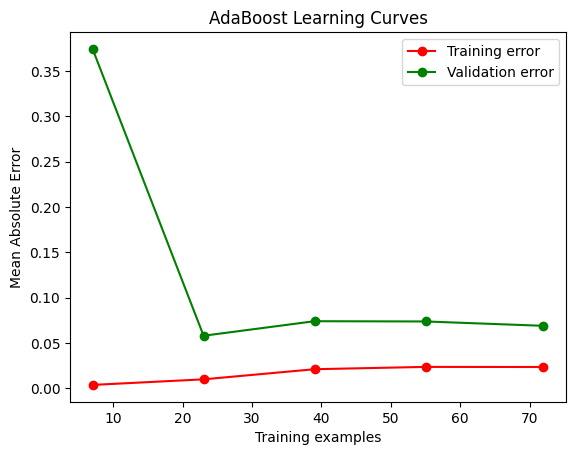
\includegraphics[width=\linewidth, trim=0 0 0 0]{images/AdaBoost_lc90_Azure.png} \\
        \hline
    \end{tabularx}
    \caption{Learning Curves con il nuovo dataset Azure con split 90/10}
    \label{tab:emissions_info}
\end{table}

\paragraph{\textbf{SVR}.}
Dal punto di vista delle metriche il regressore SVR ha ottenuto i peggiori risultati. Entrambe le learning curve diminuiscono all'aumentare delle istanze. Il modello sembra aver generalizzato da questo punto di vista, ma l'errore è ancora alto.

\paragraph{\textbf{Decision Tree Regressor}.}
Dal punto di vista delle metriche, il Decision Tree Regressor ha ottenuto i risultati secondi al Random Forest Regressor, tranne in MAE dove è il migliore.
La learning curve di validation diminuisce all'aumentare delle istanze, mentre quella di training aumenta. Il modello non ha generalizzato bene.
\paragraph{\textbf{Random Forest Regressor}.}
Dal punto di vista delle metriche il Random Forest Regressor risulta essere il miglior modello, MAE escluso. Entrambe le learning curve diminuiscono all'aumentare delle istanze. Il modello sembra aver generalizzato bene.
\paragraph{\textbf{AdaBoost Regressor}.}
Dal punto di vista delle metriche il AdaBoost Regressor ha ottenuto risultati peggiori rispetto al Decision Tree Regressor e Random Forest Regressor ma migliori rispetto al SVR.
La learning curve mostrano che il modello non è riuscito a generalizzare bene in quanto quella di validation diminuisce all'aumentare delle istanze, mentre quella di training aumenta.

\paragraph{\textbf{Conclusioni}} Questo sembra essere il miglior split per il dataset Azure. Random Forest sembra essere il miglior modello. Decision Tree è il secondo migliore. AdaBoost e SVR non sono riusciti a generalizzare bene.


\paragraph{\textbf{Conclusioni generali}}

In generale Random Forest sembra essere il miglior modello. Decision Tree `e il secondo migliore. AdaBoost e SVR non sono riusciti a generalizzare bene. In
particolare lo split dove le performance sono migliori osservando sia learning curve che metriche
`e il 90/10 a cui segue il 60/40.

\subsubsection{Confronto tra i due dataset}
Si può notare che in generale il dataset completo performa meglio del dataset di Azure.
\begin{itemize}
    \item Dataset completo: RandomForest con split 70/30
    \item Dataset Azure: RandomForest con split 90/10
\end{itemize}